\chapter{Doska Arduino}

Arduino je hardvér a softvér s otvoreným zdrojovým kódom, ktoré sú licencované na základe licencie GNPL Lesser General Public License (LGPL) alebo GNU General Public License (GPL), umožňujúce výrobu dosiek Arduino a distribúciu softvéru každým , Arduino dosky sú komerčne dostupné v predmontovanej podobe alebo v súpravách do-it-yourself.

Dosky typu Arduino používajú rôzne mikroprocesory a riadiace jednotky. Dosky sú vybavené súbormi digitálnych a analógových vstupno-výstupných (I/O) pinov, ktoré môžu byť prepojené s rôznymi rozširujúcimi doskami (shields) a inými obvodmi. Dosky obsahujú sériové komunikačné rozhrania, vrátane univerzálnej sériovej zbernice (USB) na niektorých modeloch, ktoré sa používajú aj na načítanie programov z osobných počítačov. Mikrokontroléry sú typicky naprogramované pomocou dialektu funkcií z programovacích jazykov C a C ++. Popri používaní tradičných kompilátorov poskytuje projekt Arduino integrované vývojové prostredie (IDE) založené na projekte Language Processing.

\begin{figure}[H]
	\begin{center}
		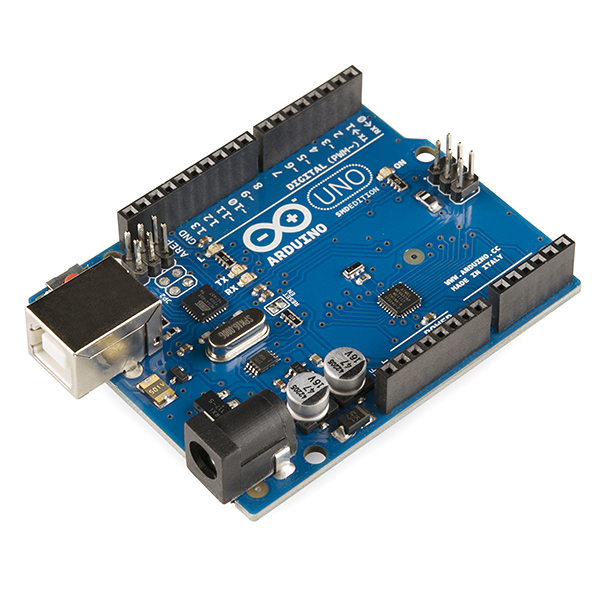
\includegraphics[height=9cm]{pics/arduino.jpg}
		\caption{Doska Arduino UNO}
		\label{pic-reference}
	\end{center}
\end{figure}


Projekt Arduino sa začal v roku 2003 ako program pre študentov v Interaction Design Institute Ivrea v Ivreu v Taliansku s cieľom poskytnúť novým a profesionálnym používateľom lacný a jednoduchý spôsob vytvárania zariadení, ktoré interagujú s prostredím pomocou senzorov a pohony. Bežné príklady takýchto zariadení určené pre začínajúcich fanatikov zahŕňajú jednoduché roboty, termostaty a detektory pohybu.

Návrhy hardvéru sú distribuované pod licenciou Creative Commons Attribution Share-Alike 2.5 a sú k dispozícii na webovej stránke spoločnosti Arduino. Sú tiež k dispozícii aj výrobné súbory pre niektoré verzie hardvéru. Zdrojový kód pre integrované vývojové prostredie (IDE) je uvoľnený pod licenciou GNU General Public License, verzia 2. Napriek tomu firmou Arduino nikdy nebol uvoľnený oficiálny zoznam materiálov Arduino.

Aj keď sú hardvérové a softvérové vzory voľne k dispozícii na základe licencií copyleft, vývojári požiadali, aby bol názov Arduino výlučne k oficiálnemu produktu a nebol použitý na odvodené diela bez povolenia. V oficiálnom dokumente o používaní názvu Arduino sa zdôrazňuje, že projekt je otvorený pre začlenenie práce iných do oficiálneho produktu. Niekoľko komerčne uvoľnených výrobkov, ktoré sú kompatibilné s Arduino, sa vyhýbali názvu projektu použitím rôznych mien končiacich v -duino.

\section{Parametre dosky}

Väčšina dosiek Arduino pozostáva z mikrokontrolera Atmel 8-bit AVR (ATmega8, ATmega168, ATmega328, ATmega1280, ATmega2560) s rôznym množstvom pamäte flash, čipov a inštrukcií. 32-bitový Arduino Due, založený na Atmel SAM3X8E bol predstavený v roku 2012. Dosky používajú jednočlenné alebo dvojradové piny alebo zásuvky, ktoré uľahčujú pripojenie na programovanie a začlenenie do iných obvodov. Môžu sa pripojiť s doplnkovými modulmi nazývanými shields. Viacnásobné a prípadne naskladané shields môžu byť individuálne adresovateľné prostredníctvom sériovej zbernice IIC. Väčšina dosiek obsahuje 5 V lineárny regulátor a 16 MHz kryštálový oscilátor alebo keramický rezonátor. Niektoré konštrukcie, ako napríklad LilyPad, pracujú na frekvencii 8 MHz a kvôli špecifickým obmedzeniam tvarových faktorov sa neuplatňujú s palubným regulátorom napätia.

\begin{figure}[H]
	\begin{center}
		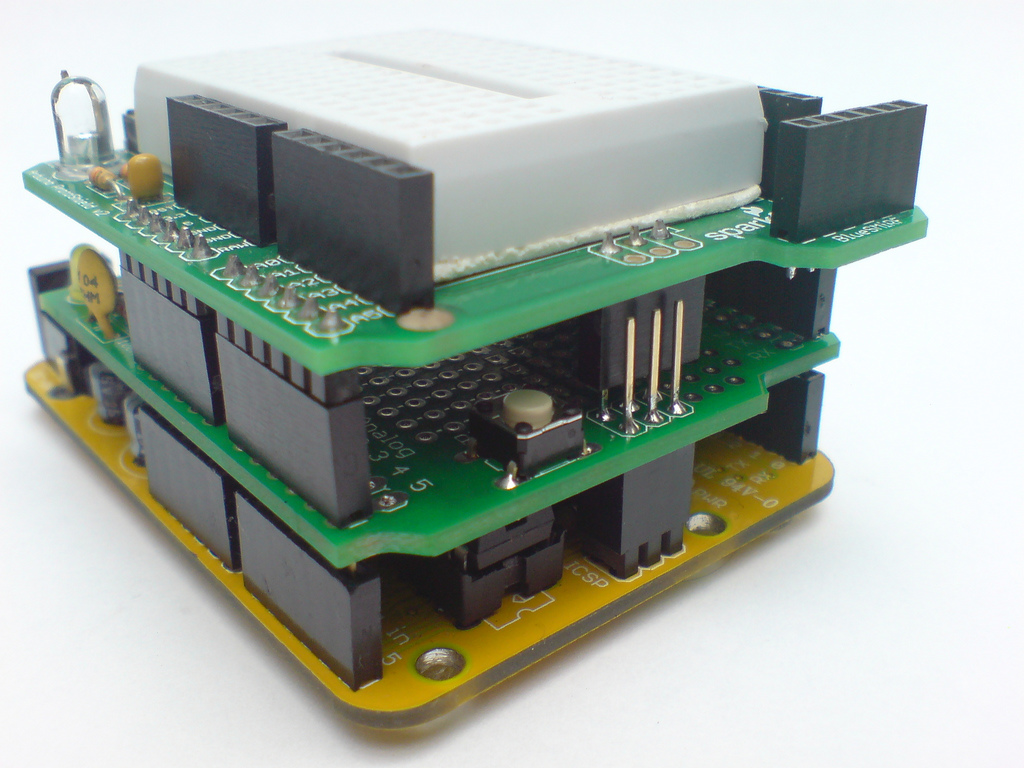
\includegraphics[height=9cm]{pics/shields.jpg}
		\caption{Viacero shields napojenych na arduino}
	\end{center}
\end{figure}

Arduino mikrokontroléry sú vopred naprogramované pomocou zavádzača, ktorý zjednodušuje nahrávanie programov do flash pamäte na čipoch. Predvolený zavádzač Aduino UNO je bootloader pre optiboot. Dosky sú načítané programovým kódom cez sériové pripojenie k inému počítaču. Niektoré sériové dosky Arduino obsahujú obvod prevodníkov úrovne na konverziu medzi logickými úrovňami RS-232 a signály úrovne TTL. Súčasné dosky Arduino sú naprogramované pomocou Universal Serial Bus (USB), ktoré sú implementované pomocou čipov typu USB-to-serial adaptérom, ako napríklad FTDI FT232. Niektoré dosky, ako napríklad neskoršie modely modelov Uno, nahradia čip FTDI samostatným čipom AVR obsahujúcim USB-to-serial firmware, ktorý je preprogramovateľný cez vlastnú hlavičku ICSP. Iné varianty, ako napríklad Arduino Mini a neoficiálny Boarduino, používajú odnímateľný USB-to-sériový adaptér alebo kábel, Bluetooth alebo iné metódy, keď sa používajú s tradičnými nástrojmi mikrokontrolérov namiesto Arduino IDE, štandardné programovanie v systéme AVR ISP).

Doska Arduino vystavuje väčšinu I / O pinov mikrokontroléra pre použitie v iných obvodoch. Arduino Uno poskytujú 14 digitálnych I / O pinov, z ktorých šesť môže produkovať signály modulované šírkou pulzu a šesť analógových vstupov I / O pinov. Tieto piny sa nachádzajú na hornej časti dosky pomocou zásuviek s priemerom 0,1 palca (2,54 mm). Niektoré zásuvné aplikácie sú komerčne dostupné. Dosky Arduino Nano môžu poskytovať zástrčky na spodnej strane dosky, ktoré sa môžu pripojiť do bezpájkových lôk.

\section{Rôzne typy dosiek}

Existuje mnoho dosiek odvodených od Arduino a Arduino. Niektoré sú funkčne ekvivalentné s Arduino a môžu byť použité zameniteľné. Mnohé zdokonaľujú základné Arduino tým, že pridávajú výstupné ovládače, často používané v školskom vzdelávaní, aby zjednodušili výrobu kočíkov a malých robotov. Ostatné sú elektricky ekvivalentné, ale menia tvarový faktor, niekedy si zachovávajú kompatibilitu so štítmi. Niektoré varianty používajú rôzne procesory s rôznou kompatibilitou.

\begin{figure}[H]
	\begin{center}
		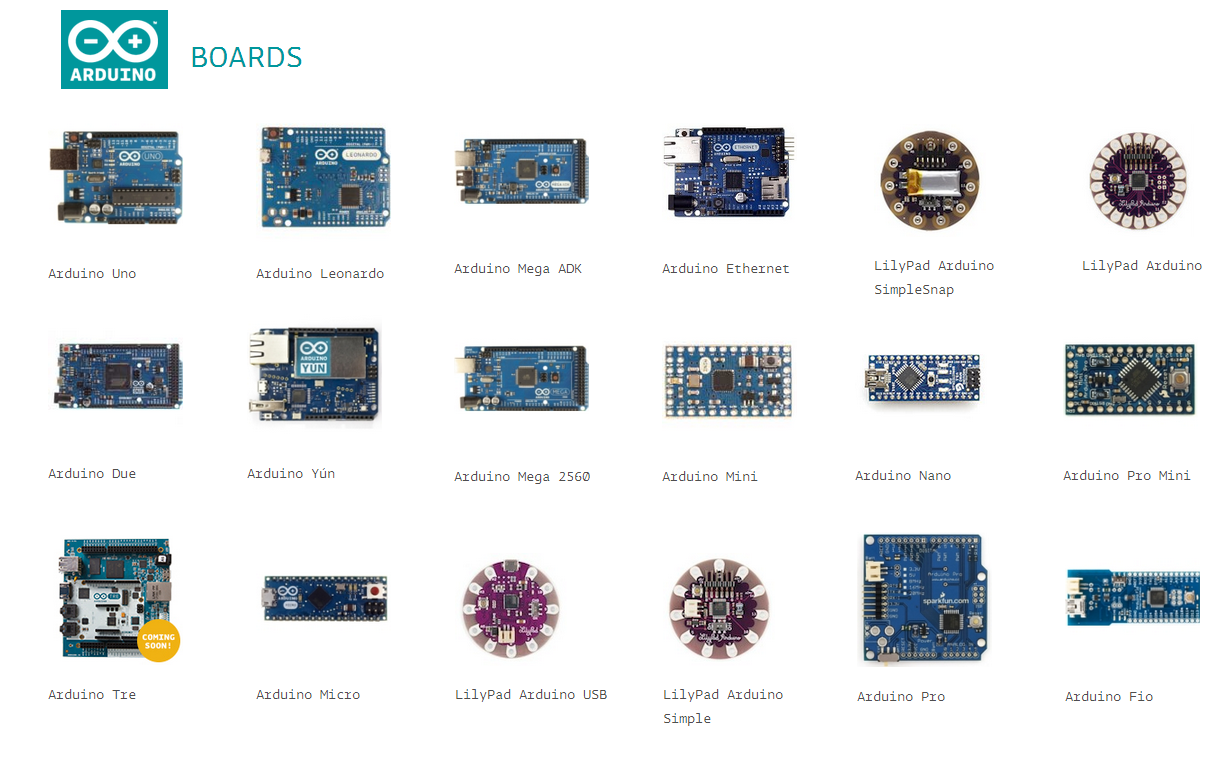
\includegraphics[height=9cm]{pics/arduino-boards.png}
		\caption{Príklady dosiek}
	\end{center}
\end{figure}

\chapter{Elektronicé komponenty}

Existuje mnozstvo komponentov s ktorymi sa stretávame každodenne. Či už s tlačidlom na ovládači, LED diódov alebo potenciometrom pri úprave hlasitosti v aute, a pod. Všetky tieto komponenty majú popis fungovania. Preto sa v práci pokúsime pripraviť balík základných komponentov. Na obrázku si môžeme pozrieť ako také komponenty vyzerajú.

\begin{figure}[H]
	\begin{center}
		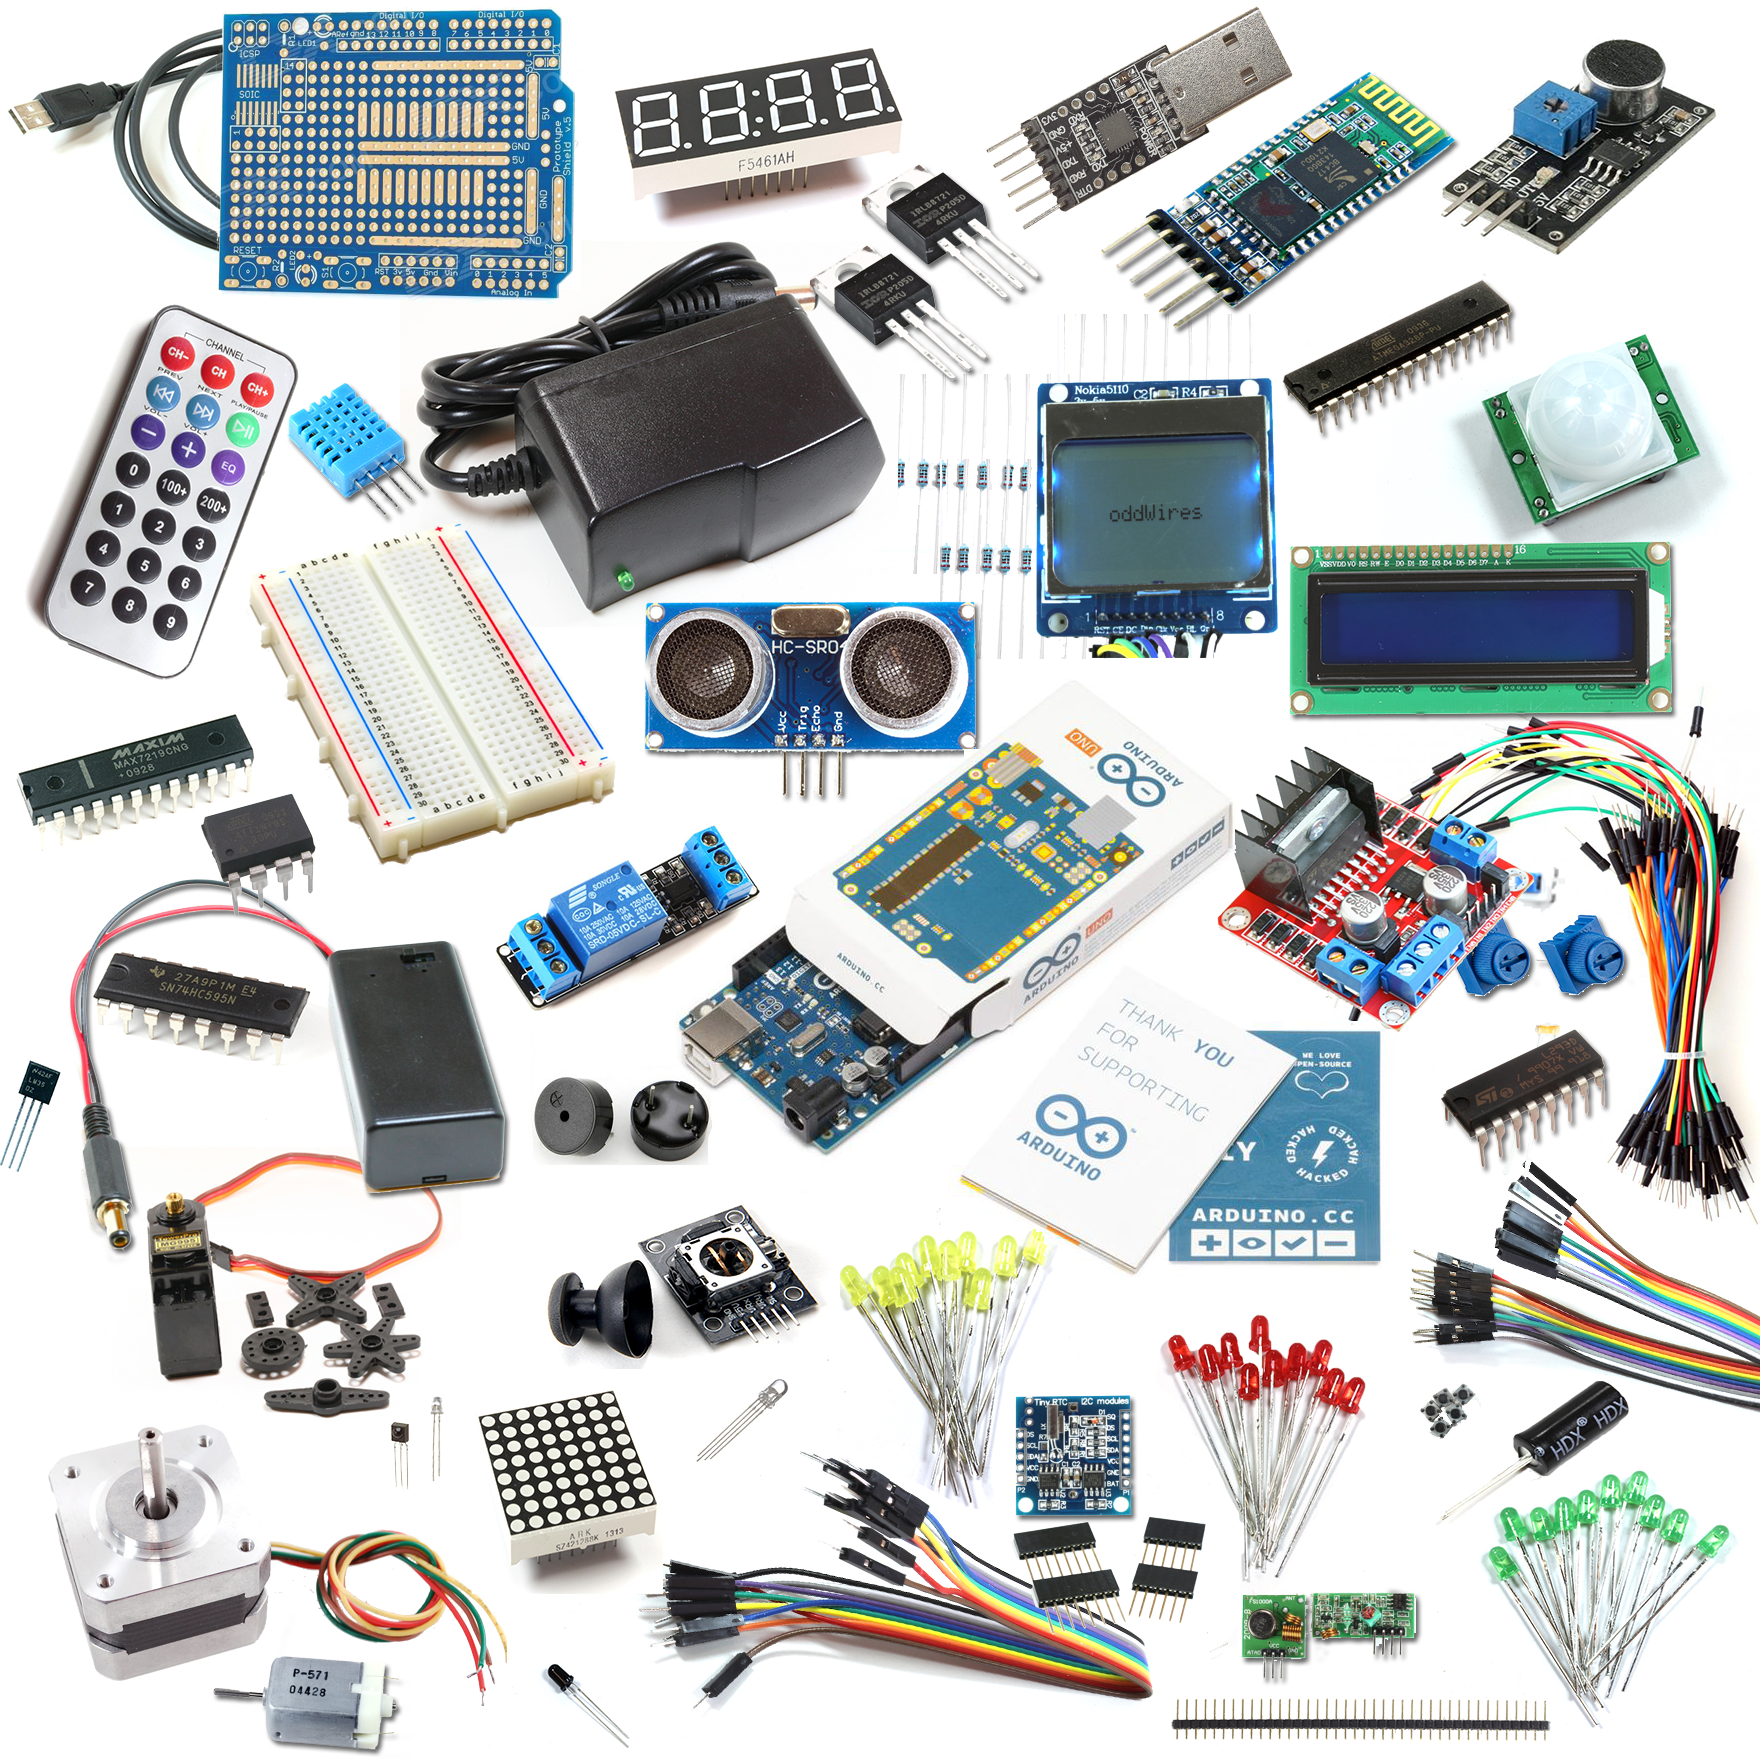
\includegraphics[height=9cm]{pics/components.png}
		\caption{Príklady rôznych elektronických komponentov}
	\end{center}
\end{figure}


\chapter{Integrované vývojové prostredie}

Integrované vývojové prostredie (IDE) je softvérová aplikácia, ktorá poskytuje komplexné vybavenie pre programátorov pre vývoj softvéru. IDE sa zvyčajne skladá z editora zdrojového kódu, nástrojov na tvorbu automatizácie a nástroja na ladenie. Väčšina moderných IDE má inteligentné dokončenie kódu. Niektoré IDE, ako napríklad NetBeans a Eclipse, obsahujú kompilátor, interpret alebo oboje; Iné, napríklad SharpDevelop a Lazarus, nie. Hranica medzi integrovaným vývojovým prostredím a inými časťami širšieho prostredia vývoja softvéru nie je dobre definovaná. Niekedy je integrovaný systém riadenia verzií alebo rôzne nástroje na zjednodušenie konštrukcie Grafického používateľského rozhrania (GUI). Mnoho moderných IDE má tiež triedny prehliadač, prehliadač objektov a hierarchický diagram triedy pre použitie v objektovo-orientovanom vývoji softvéru.

\begin{figure}[H]
	\begin{center}
		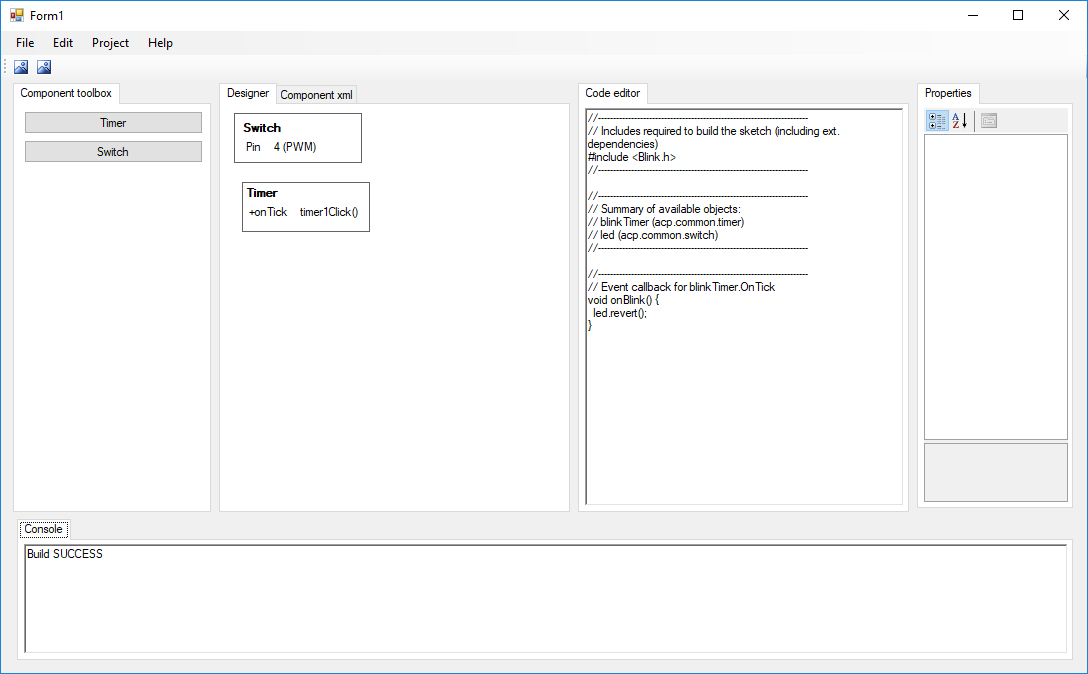
\includegraphics[height=9cm]{pics/ide.png}
		\caption{Príklad IDE pre naše riešenie}
	\end{center}
\end{figure}

\chapter{Podobné riešenia}
Stále rastúca komunita sa venuje zariadeniam Arduino. S tým je spojený aj vývoj rôznych frameworkov pre túto platformu, ktorých cieľom je zjednodušiť vývoj programátorom. Riešenia aké sme s pomocou Arduino komunity našli, rozdeľujeme do kategórií online a offline. Online sú riešenia, ktoré do zariadenia nainštalujú zavádzač preposielajúci a vykonávajúci akcie len od servera (logika systému je len na serveri). Offline sú riešenia bežiace priamo na Arduino zariadení a na vykonanie akcie sa rozhodujú bez servera. Nižšie si povieme niečo viac o jednom online a dvoch offline riešeniach. Všetky existujúce riešenia šli viac smerom automatov, alebo len udalostí.

\section{Arduino EventManager}
Je offline riešenie v ktorom neprogramujeme hlavné vlákno loop(). Programujeme však spracovanie udalostí. Na začiatku programu pre EventManager potrebujeme určiť, na zmeny ktorých pinov cheme vyvolať udalosť. Následne ak zmena nastane EventManager túto udalosť vykoná.

\begin{algorithm}[H]
	\caption{Príklad použitia EventManager.}\label{alg-euclid}
	\begin{verbatim}
		void myListener( int eventCode, int eventParam )
		{
			// Do something with the event
		}

		void setup()
		{
			gMyEventManager.addListener( EventManager::kEventUser0, myListener );

			// Do more set up
		}
	\end{verbatim}
\end{algorithm}


\section{Quantum Leaps Modeling Tool}
Je offline riešenie spolu s modelovacím nástrojom. Toto riešenie je špecifické tým, že pristupuje k programovaniu ako k stavovému automatu. Konečno stavový automat je matematický model výpočtu. Je to abstraktný stroj, ktorý môže byť v danom čase presne v jednom stave z konečného počtu stavov. Konečno stavový automat sa môže zmeniť z jedného stavu na druhý v reakcii na niektoré externé vstupy. Je definovaný zoznamom jeho stavov, ich počiatočným stavom a podmienkami pre každý prechod.

\begin{figure}[H]
	\begin{center}
		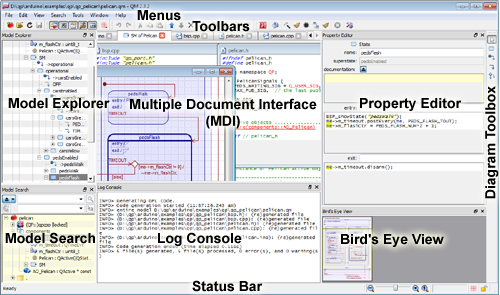
\includegraphics[height=9cm]{pics/qm.png}
		\caption{Príklad IDE pre naše riešenie}
	\end{center}
\end{figure}

\section{Cayenne}

Je online riešenie podporujúce mnoho Arduino dosiek, kde každá doska posiela na server aktuálny stav pinov. Vyhodou tohto riešenia je priateľské používateľské prostredie s jednoduchým nastavením prahov pre jednotlivé piny Arduino dosiek, s priradením následnej akcie. Napr. Ak stúpne teplota (teplotný senzor je na pine 5) nad 30C, tak zapni klimatizáciu (zapni 5V na pine 4).

\begin{figure}[H]
	\begin{center}
		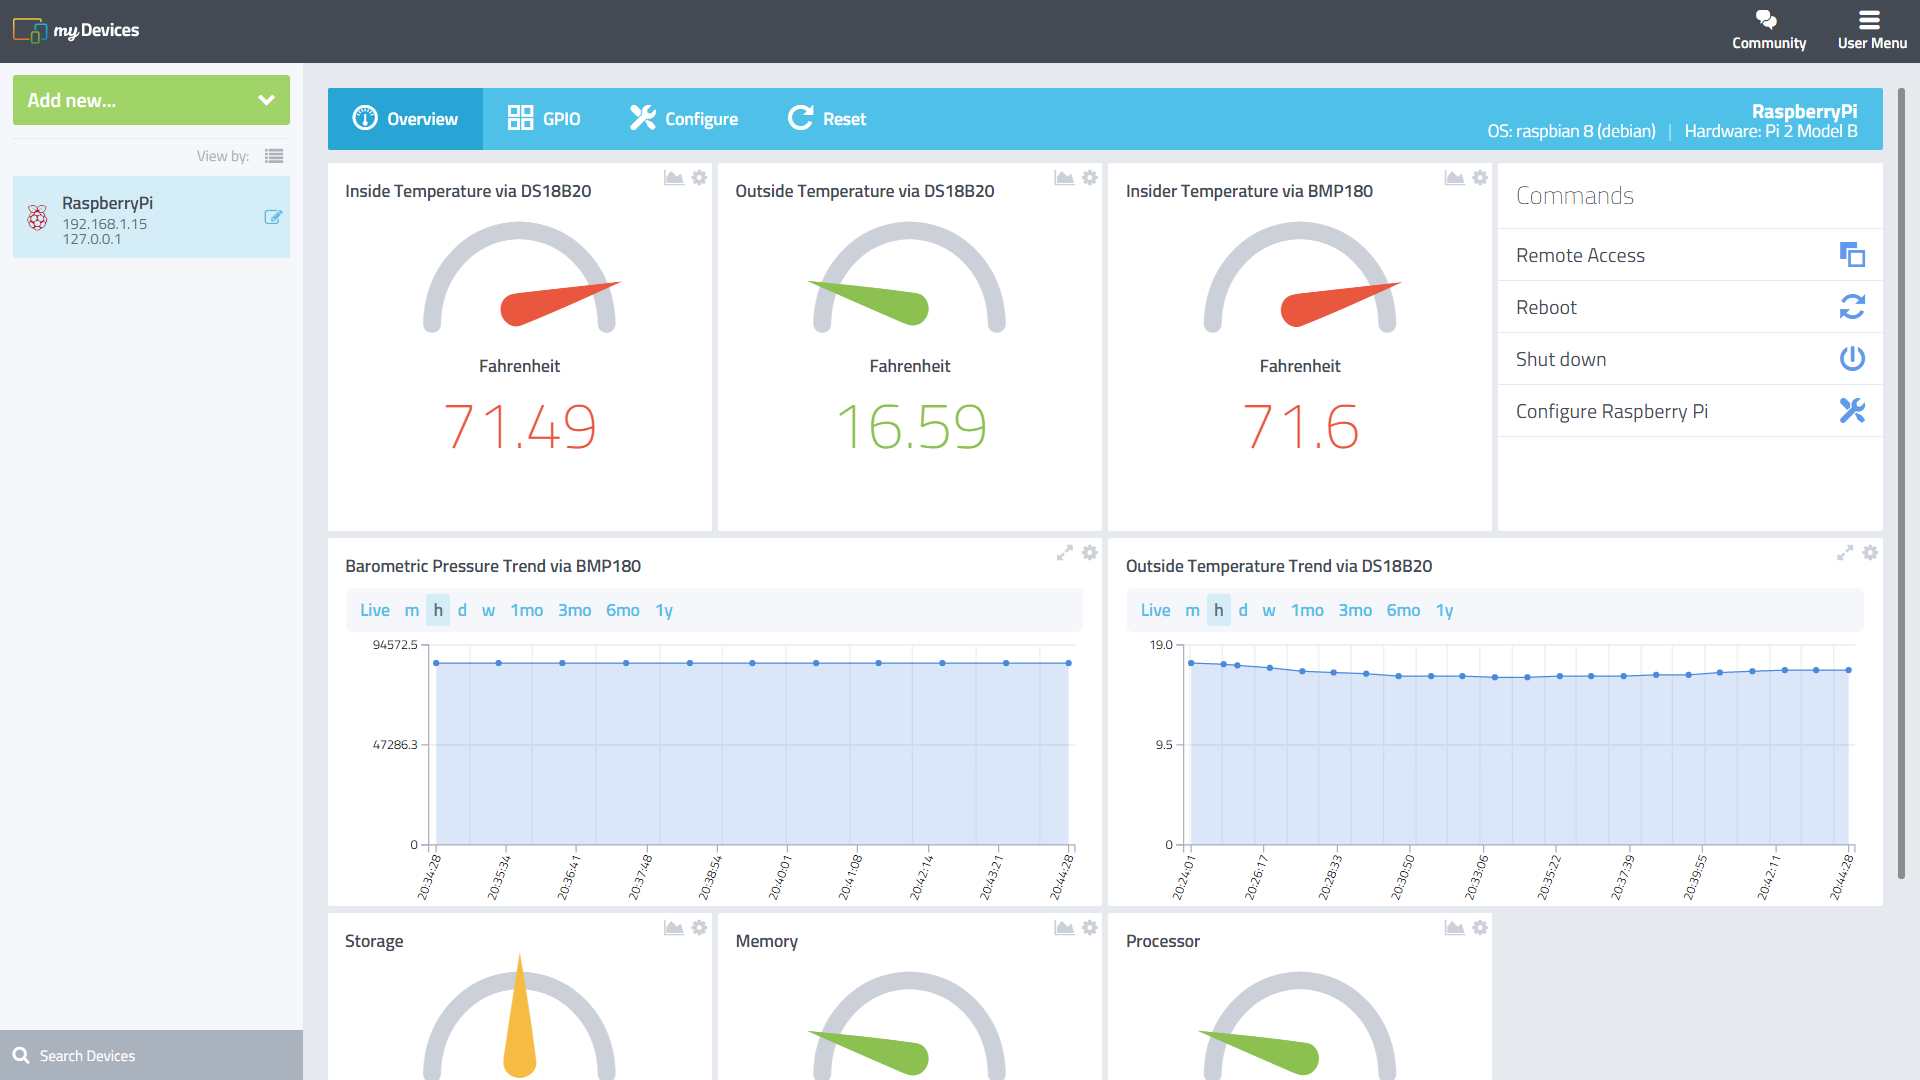
\includegraphics[height=9cm]{pics/cayenne.png}
		\caption{Príklad IDE pre naše riešenie}
	\end{center}
\end{figure}


\chapter{Postup práce}
Naším prvým krokom je vývoj plánovača úloh pre komponenty, ktorý bude vedieť efektívne a v reálnom čase vykonávať udalosti vytvorené komponentami. Znova si musíme uvedomiť, že máme k dispozícii iba 2048 B operačnej pamäte. Ďalším faktom je, že čím viac pamäte spotrebuje plánovač úloh, tým menej komponentov budeme môcť použiť. To znamená, že v prípade, ak by sme využili celú pamäť pre plánovač, tak vieme iba plánovať a nemôžeme urobiť nič viac. Preto sa pri návrhu zameriame na využitie čo najmenšej časti tejto operačnej pamäte.

Spolu s vývojom plánovača vytvoríme aj základné komponenty:

\begin{itemize}
\item Časovač – komponent, ktorý bude v zadanom intervale spúšťať preddefinované udalosti
\item Prepínač – komponent, ktorý bude zapínať alebo vypínať port zo zariadenia, napríklad zapne/vypne Led diódu
\item Senzor – komponent, ktorý bude sledovať port zariadenia, v ktorom je pripojený senzor: ak sa na senzore zmení hodnota, tak spustí definovanú udalosť (napríklad po stlačení tlačidla sa vykoná zapnutie Prepínača)
\end{itemize}

Pri tvorbe musíme - rovnako ako pri tvorbe plánovača úloh -  dbať na veľkosť operačnej pamäte (2048 B). 

To, čo otvorilo dvere zariadeniam Arduino, bolo práve vývojové prostredie Arduino IDE. Preto sa v ďalšej kapitole budeme venovať tvorbe vývojového prostredia podobného tomu, ktoré sme použili pri vývoji Swing aplikácií. V našom prostredí bude používateľ kliknutím vytvárať jednotlivé komponenty, ktorým nastaví jednotlivé parametre. Z týchto dát sa automaticky vygeneruje zdrojový kód pre plánovač úloh. Pri návrhu vývojového prostredia a generátora kódu musíme dbať na budúcu rozšíriteľnosť dostupných typov komponentov. V tejto kapitole sa prevažne budeme venovať 


\begin{itemize}
\item analýze zdrojového kódu z pohľadu párovania parametrov z komponentov ku zdrojovým kódom
\item analýze kódu z pohľadu hľadania kolízií, kde bude viac komponentov súčasne používať tie isté prostriedky
\item problematike kompilátora pre tieto zariadenia
\end{itemize}

Posledným krokom bude implementácia ďalších bežne používaných komponentov, kde pri vývoji sa budeme znova riadiť všetkými už spomenutými podmienkami.

\cite{iot1}, \cite{iot2}, \cite{iot3}